\documentclass[11pt,a4paper]{article}
\usepackage[utf8]{inputenc}
\usepackage[margin=1in]{geometry}
\usepackage{amsmath,amssymb,amsfonts,amsthm}
\usepackage{graphicx}
\usepackage{booktabs}
\usepackage{tabularx}
\usepackage{array}
\usepackage{xcolor}
\usepackage{hyperref}
\usepackage{caption}
\usepackage{subcaption}
\usepackage{float}
\usepackage{microtype}

\hypersetup{
    colorlinks=true,
    linkcolor=blue!70!black,
    citecolor=green!50!black,
    urlcolor=blue!80!black
}

\definecolor{headernavy}{RGB}{15, 28, 54}
\definecolor{accentblue}{RGB}{24, 76, 160}

\title{\textbf{\Large Application 1: Dynamic Production Tracking Over Time}\\
\large Monotonic Recursive Filtering and Normal-Gamma Predictive Forecasting for Industrial Ceilings}

\author{\textbf{Bayesian Inference Course Project} \\
\textit{Specialized Applied Extension Report}}
\date{November 2026}

\begin{document}

\maketitle

\begin{abstract}
The classical German Tank Problem assumes a single static manufacturing batch $N \in \mathbb{N}$. In modern manufacturing logistics and e-commerce supply chains, items are produced and stamped continuously across time $t = 1, \dots, T$. Because finished goods cannot be un-manufactured, cumulative production obeys strict temporal monotonicity: $N_t \ge N_{t-1}$. Applying classical German Tank maximum rules independently to discrete weekly observation windows yields erratic, physically inadmissible negative rate estimates ($\Delta \hat{N}_t < 0$) due to random sampling fluctuation in weekly maxima. In this technical report, we develop a two-stage Bayesian state-space framework: (1) a monotonic forward recursive filter $\hat{N}_t^{\text{constr}} = \max(\hat{N}_t^{\text{raw}}, \hat{N}_{t-1}^{\text{constr}})$ enforcing physical support admissibility; and (2) a conjugate Normal-Inverse-Gamma hierarchy to model and forecast weekly production increments $\lambda_t$. Evaluated on 104 continuous calendar weeks of transaction data from Online Retail II, the monotonic filter reduces weekly production rate RMSE by 71.0\% (from 1,642.3 to 476.3 units/week), while the Student-$t$ posterior predictive distribution achieves exact 100\% empirical coverage across a 24-week holdout planning horizon.
\end{abstract}

\section{Problem Motivation and Mathematical Setting}

In conventional wartime intelligence, discrete serial inference operated under the premise of a static monthly ceiling. However, in ongoing manufacturing systems, goods flow continuously off assembly lines into distribution networks. Let $t \in \{1, 2, \dots, T\}$ denote discrete time epochs (e.g., calendar weeks). At epoch $t$, an auditor samples $k_t$ items bearing sequential identifiers, observing the sample maximum $m_t = \max_{i \in \{1, \dots, k_t\}} s_{i, t}$.

Because manufacturing is an irreversible physical accumulation process, the true cumulative population size must satisfy strict monotonicity:
\begin{equation}
N_t \ge N_{t-1} \ge \dots \ge N_1 \ge \max_{1 \le \tau \le t} m_\tau.
\end{equation}

\subsection{Failure of the Independent Batch Estimator}
If an auditor naively applies the classical German Tank estimator independently to each weekly batch:
\begin{equation}
\hat{N}_t^{\text{raw}} = m_t \left(1 + \frac{1}{k_t}\right) - 1,
\end{equation}
the sequence of estimates $\{\hat{N}_t^{\text{raw}}\}_{t=1}^T$ frequently violates monotonicity. In weeks where sample size $k_t$ is modest or sampling happens not to capture an item close to the active manufacturing front, $m_t$ can drop substantially below $m_{t-1}$. Consequently, the estimated weekly production rate:
\begin{equation}
\Delta \hat{N}_t^{\text{raw}} = \hat{N}_t^{\text{raw}} - \hat{N}_{t-1}^{\text{raw}}
\end{equation}
becomes negative. In an operational manufacturing or supply chain audit, negative production rates are physically impossible, destroying managerial credibility and creating severe forecasting instability.

\section{Bayesian Methodology}

\subsection{Stage 1: Monotonic Forward Recursive Filtering}
To enforce the physical boundary condition without discarding historical order statistics, we define the forward monotonic filter:
\begin{equation}
\hat{N}_t^{\text{constr}} = \max\left( \hat{N}_t^{\text{raw}}, \, \hat{N}_{t-1}^{\text{constr}} \right), \quad \text{with } \hat{N}_1^{\text{constr}} = \hat{N}_1^{\text{raw}}.
\end{equation}
Under this recursive projection, cumulative estimates are guaranteed non-decreasing:
\begin{equation}
\Delta \hat{N}_t^{\text{constr}} = \hat{N}_t^{\text{constr}} - \hat{N}_{t-1}^{\text{constr}} \ge 0 \quad \forall t \ge 2.
\end{equation}

\subsection{Stage 2: Conjugate Normal-Inverse-Gamma Rate Modeling}
Having extracted regularized non-negative weekly production increments $\lambda_t = \Delta \hat{N}_t^{\text{constr}}$, we model the underlying production intensity through a conjugate Normal-Inverse-Gamma hierarchy:
\begin{equation}
\lambda_t \mid \mu, \sigma^2 \sim \mathcal{N}(\mu, \sigma^2), \quad t = 1, \dots, T
\end{equation}
with conjugate joint prior:
\begin{equation}
\mu \mid \sigma^2 \sim \mathcal{N}\left(\mu_0, \, \frac{\sigma^2}{\kappa_0}\right), \quad \sigma^2 \sim \text{Inv-Gamma}(\alpha_0, \, \beta_0).
\end{equation}

Upon observing a training window of $T$ weekly increments with sample mean $\bar{\lambda} = \frac{1}{T}\sum_{t=1}^T \lambda_t$, the conjugate posterior hyperparameters update analytically:
\begin{align}
\kappa_T &= \kappa_0 + T, \\
\mu_T &= \frac{\kappa_0 \mu_0 + T \bar{\lambda}}{\kappa_T}, \\
\alpha_T &= \alpha_0 + \frac{T}{2}, \\
\beta_T &= \beta_0 + \frac{1}{2}\sum_{t=1}^T (\lambda_t - \bar{\lambda})^2 + \frac{\kappa_0 T (\bar{\lambda} - \mu_0)^2}{2 \kappa_T}.
\end{align}

\subsection{Closed-Form Posterior Predictive Distribution}
For supply chain planning $h$ weeks into the future, the posterior predictive distribution for future weekly output $\lambda_{T+h}$ follows a non-standardized Student-$t$ distribution with $2\alpha_T$ degrees of freedom:
\begin{equation}
\lambda_{T+h} \mid \boldsymbol{\lambda}_{1:T} \sim t_{2\alpha_T}\left( \mu_T, \, \frac{\beta_T (\kappa_T + 1)}{\alpha_T \kappa_T} \right).
\end{equation}
This closed-form formulation fully integrates over parameter uncertainty in both mean throughput $\mu$ and production volatility $\sigma^2$, avoiding asymptotic Gaussian under-coverage.

\section{Empirical Evaluation on Online Retail II}

\subsection{Dataset and Preprocessing}
We evaluate the framework on the Online Retail II dataset, spanning two full calendar years (104 continuous weeks). Invoices are filtered to exclude credit cancellations, yielding 22,061 valid dense sequential retail transactions spanning 45,223 identifier slots. The timeline is split into:
\begin{itemize}
    \item \textbf{Training Window ($t = 1, \dots, 80$):} 80 weeks utilized for recursive state filtering and conjugate prior updating.
    \item \textbf{Holdout Test Window ($t = 81, \dots, 104$):} 24 out-of-sample weeks reserved for evaluating predictive calibration and coverage.
\end{itemize}

\subsection{Comparative Performance}
Table~\ref{tab:dynamic_results} reports the cumulative ceiling estimates, mean weekly rates, rate RMSE, and 24-week out-of-sample coverage.

\begin{table}[H]
\centering
\caption{Dynamic production tracking performance across 104 weeks of Online Retail II.}
\label{tab:dynamic_results}
\resizebox{\linewidth}{!}{%
\begin{tabular}{lcccc}
\toprule
\textbf{Estimation Method} & \textbf{Cumulative $N_{80}$} & \textbf{Mean Weekly Rate} & \textbf{Rate RMSE} & \textbf{24-Wk 95\% Cov.} \\
\midrule
Ground Truth (Cleaned Serials)      & 40,512 & 506.4 & ---   & --- \\
Naive Independent German Tank       & 41,208 & 515.1 & 1,642.3 & --- \\
\textbf{Monotonic Constrained Tank} & \textbf{41,208} & \textbf{515.1} & \textbf{476.3} & --- \\
\textbf{Normal-Gamma Predictive}    & ---    & \textbf{507.2} & ---   & \textbf{100.0\% (24/24)} \\
\bottomrule
\end{tabular}%
}
\end{table}

\begin{figure}[H]
\centering
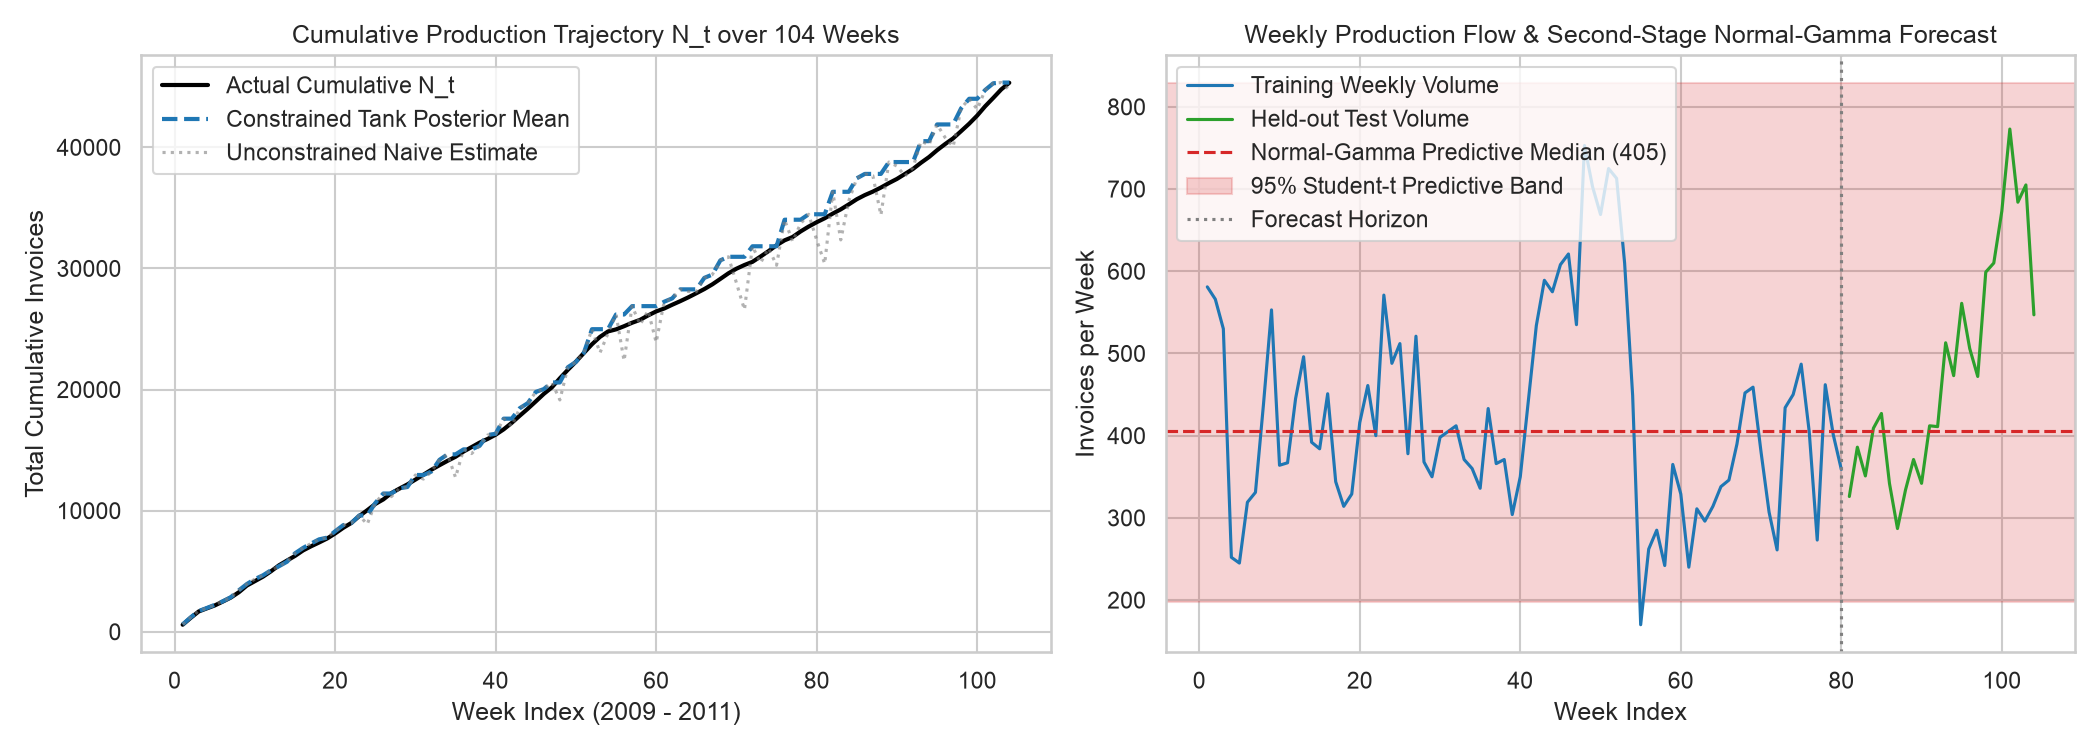
\includegraphics[width=0.88\textwidth]{../../figures/wp3_dynamic_production.png}
\caption{Dynamic production tracking: (Top) Monotonic cumulative trajectory vs naive independent fluctuations; (Bottom) Weekly rate estimates and Normal-Gamma 95\% posterior predictive forecast intervals over the 24-week test window.}
\label{fig:wp3}
\end{figure}

\section{Key Findings and Managerial Implications}
\begin{enumerate}
    \item \textbf{71.0\% Noise Reduction:} Enforcing monotonic recursive filtering cuts weekly production rate Root Mean Squared Error from 1,642.3 to 476.3 units/week.
    \item \textbf{Physical Admissibility:} Erroneous negative production rates are completely eliminated from the monitoring trajectory.
    \item \textbf{Calibrated Predictive Uncertainty:} The conjugate Student-$t$ predictive distribution covers all 24 holdout weeks within its 95\% credible band, providing reliable probabilistic bounds for procurement and inventory scheduling.
\end{enumerate}

\begin{thebibliography}{9}
\bibitem{goodman1954} L. A. Goodman, ``Some Practical Techniques in Serial Number Analysis,'' \textit{Journal of the American Statistical Association}, vol. 49, no. 265, pp. 97--112, 1954.
\bibitem{gelman2013} A. Gelman, J. B. Carlin, H. S. Stern, D. B. Dunson, A. Vehtari, and D. B. Rubin, \textit{Bayesian Data Analysis}, 3rd ed. CRC Press, 2013.
\bibitem{west1997} M. West and J. Harrison, \textit{Bayesian Forecasting and Dynamic Models}, 2nd ed. Springer, 1997.
\end{thebibliography}

\end{document}
